\chapter{Channel Coding \& System Performance} \label{ch:coding}

To enhance system robustness against the adverse conditions of the acoustic channel, we implement a Forward Error Correction (FEC) strategy. While this introduces a trade-off in terms of reduced throughput and increased computational complexity, it is essential for maintaining a reliable link in low SNR regimes.

\section{Concatenated FEC Architecture} \label{sec:FEC_Architecture}

The architecture follows a classical hierarchical structure, employing an outer block code and an inner convolutional code. See \textcite{LinCostello2004}. This configuration is synergistic: the inner decoder suppresses the noise floor, while the outer decoder cleans up the residual error bursts that often escape the inner stage.

\begin{definition}[Concatenated Code Specification]
    The implemented scheme consists of two layers:
    \begin{itemize}
        \item \textbf{Outer Code:} A Reed-Solomon (RS) block code with parameters $(n,k) = (255, 239)$ operating on $m=8$-bit symbols. This code can correct up to $t=8$ symbol errors per block.
        \item \textbf{Inner Code:} A convolutional code with rate $R=1/2$ and constraint length $K=7$. It utilizes the standard generator polynomials $G_1 = 171_8$ and $G_2 = 133_8$.
    \end{itemize}
    This results in a net coding rate of approximately $R_{net} \approx 0.47$, prioritizing reliability over spectral efficiency.
\end{definition}

\begin{figure}[!ht]
    \fcapside[\FBwidth]{%
        \captionsetup{parskip = .5\baselineskip plus 1pt}%
        \caption[BER Performance Comparison]{%
            Bit Error Rate (BER) versus SNR.
            The plot illustrates the \enquote{coding gain} achieved by the concatenated scheme. The waterfall region typically begins around 10 dB, where the Viterbi decoder becomes effective against random noise.
        }%
        \label{fig:ber_fec}%
    }{%
        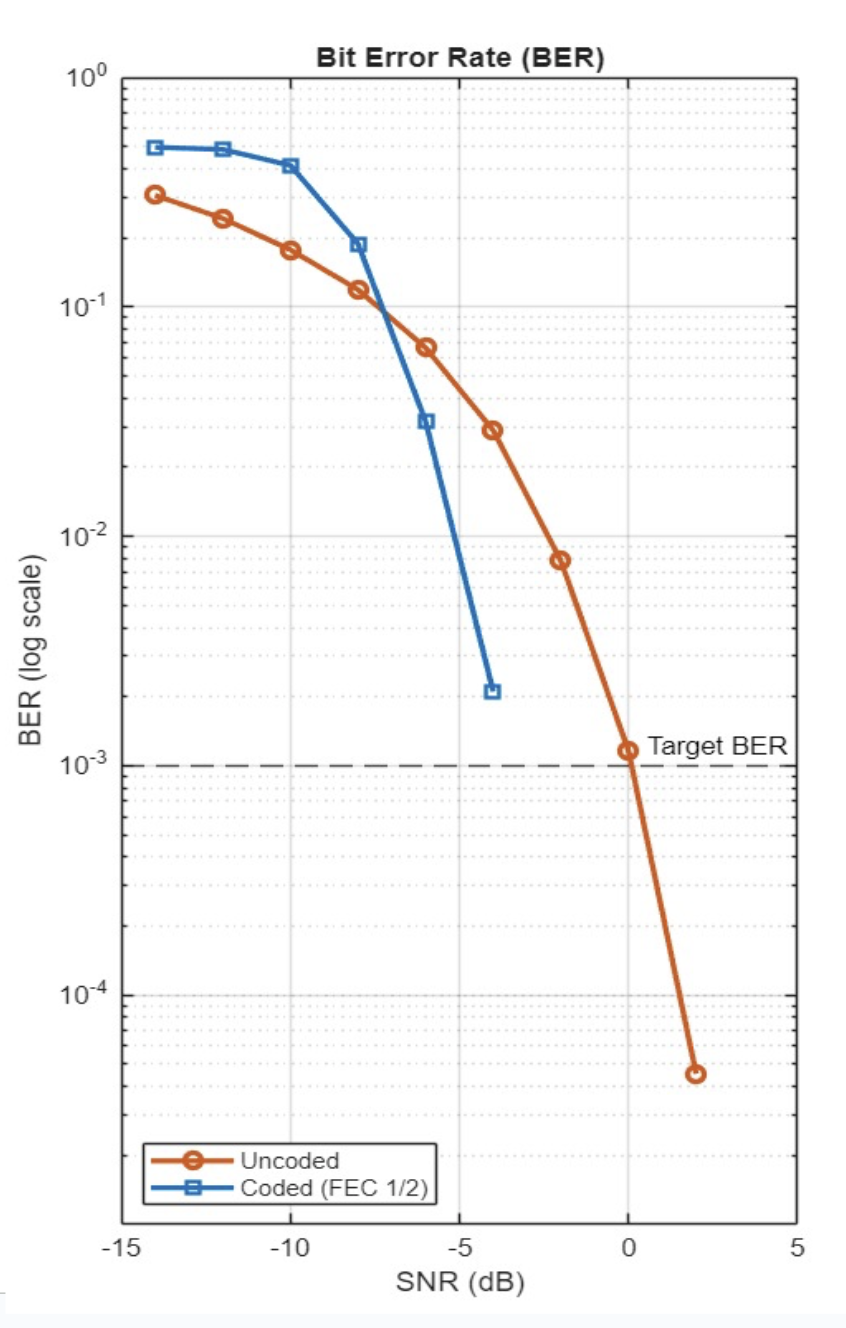
\includegraphics[width=0.45\textwidth]{figures/chap4_performance/Spectral_Efficiency_BER.png}
    }
\end{figure}

\section{Implementation Logic} \label{sec:Coding_Implementation}

The data processing flow is orchestrated by the \path{custom_function/transmit/channel_encoder.m} and \path{custom_function/receive/channel_decoder.m} scripts. These functions manage the alignment between the bit-level operations of the convolutional code and the symbol-level operations of the RS code.

\subsection{Encoding Process}

At the transmitter, the payload bits undergo a strict formatting sequence:
\begin{enumerate}
    \item \textsf{Symbol Alignment:} Input bits are padded to ensure the total length is a multiple of $m=8$, then converted into integer symbols.
    \item \textsf{Outer Encoding:} The \path{rsenc} function processes blocks of $k=239$ symbols, appending parity data to form $(n,k)$ codewords.
    \item \textsf{Inner Encoding:} The symbol stream is serialized back into bits and passed through the \path{convenc} function, generating the final redundant bitstream for modulation.
\end{enumerate}

\subsection{Decoding and Recovery}

The receiver performs the inverse operations with specific safeguards to maximize data integrity. The inner decoding uses the Viterbi algorithm (\path{vitdec}) in \emph{hard-decision} mode, with a traceback depth defined by \path{conf.coding.traceBackDepth} (typically $5K$ to $7K$).

\begin{remark}[Fallback Mechanism]
    A critical feature of our \path{channel_decoder.m} is the robustness against decoding failures.
    If the Reed-Solomon decoder detects more errors than its correction capability $t$, it typically fails.
    In our implementation, we catch this failure and extract the \emph{systematic part} of the block (the raw data symbols) instead of discarding the frame entirely. This allows upper layers to potentially recover partial information.
\end{remark}

\section{Performance Analysis} \label{sec:Performance_Analysis}

The impact of the FEC chain is quantified in \Cref{fig:ber_fec}. The transition from uncoded to coded transmission yields a significant coding gain.
In the acoustic channel, where multipath fading creates severe spectral nulls, the uncoded BER curve often flattens (error floor). The concatenated code effectively lowers this floor.

\begin{Note}[Hard vs. Soft Decision]
    The current implementation utilizes \emph{hard-decision} Viterbi decoding.
    Transitioning to \emph{soft-decision} decoding—passing confidence levels from the demodulator to the decoder—would theoretically yield an additional gain of 2 dB to 3 dB, though at the cost of increased memory usage and complexity.
\end{Note}

\Cref{tab:coding_summary} summarizes the trade-offs observed during system characterization.

\begin{table}[!ht]
    \centering
    \small
    \begin{tblr}{
        colspec = {X[l,m] X[c,m] X[c,m]},
        hlines, vlines,
        row{1} = {bg=gray!15, font=\sffamily\bfseries}
    }
        Metric & Uncoded System & Coded System \\
        Primary Error Type & Random Bit Flips & Residual Symbol Bursts \\
        Spectral Efficiency & High ($1.0 \times$ rate) & Low ($\approx 0.47 \times$ rate) \\
        Throughput @ High SNR & Max & Reduced \\
        Throughput @ Low SNR & Near Zero (Packet Loss) & Maintained \\
        Decoder Complexity & Negligible & High (Viterbi + RS) \\
    \end{tblr}
    \caption[Coding Trade-offs]{Comparison of link characteristics with and without the Concatenated FEC scheme.}
    \label{tab:coding_summary}
\end{table}